%\graphicspath{ {./content/simu/figure/} }

\section{\acl{ndt} based on punctual excitation}\label{sec:3}

\subsection{Non-through defect detection}\label{subsec:31}

In this section, the concept used to detect defect is presented and validated through simulation. Then, a specific image processing algorithm is developed to analyze the thermal evolution of each heated point. 

\subsubsection{Simulation}\label{subsec:311}

A 3D transient analysis is developed on COMSOL\textsuperscript{$\copyright$} software using \ac{fem}. The test object is a steel plate with \SI{10}{\milli \metre} thickness with the following properties: one face is flat while the other is degraded by non-through holes of \SI{10}{\milli \metre} diameter drilled at different depths. A thermal simulation including thin insulating layer subjected to laser irradiation is carried out. 
A conductive heat transfer within the metal medium is simulated through the time dependent partial differential equation such as:

\begin{equation}
  \label{eq:1}
  \rho C_p \frac{\partial T}{\partial t} = \nabla \left[ k \nabla T  \right] + Q \ ,
\end{equation}

\noindent where $\rho$ is material density, $C_p$ is specific heat capacity, $T$ is temperature, $t$ is time, $k$ is thermal conductivity and $Q$ is a heat source term.
In our simulation, $Q$ has been set to $0$ and the metal medium is considered as opaque. The laser heat source is considered as an inward heat flux and characterized by a Gaussian distribution such as:

\begin{equation}
  \label{eq:2}
  q_0 = \left( 2 \frac{P_L}{\pi r_{0}^{2}} \right) \exp \left( -2 \left( \frac{x^2 + y^2}{r_{0}^{2}} \right) \right) \ ,
\end{equation}

\noindent where $P_L$ is the laser power, $r_0$ is the laser beam waist, $x$ and $y$ are spatial coordinates.
%
\begin{figure}
  \centering
	
	
  \hspace*{\fill}
	\subfigure[]{\label{subfig:2a}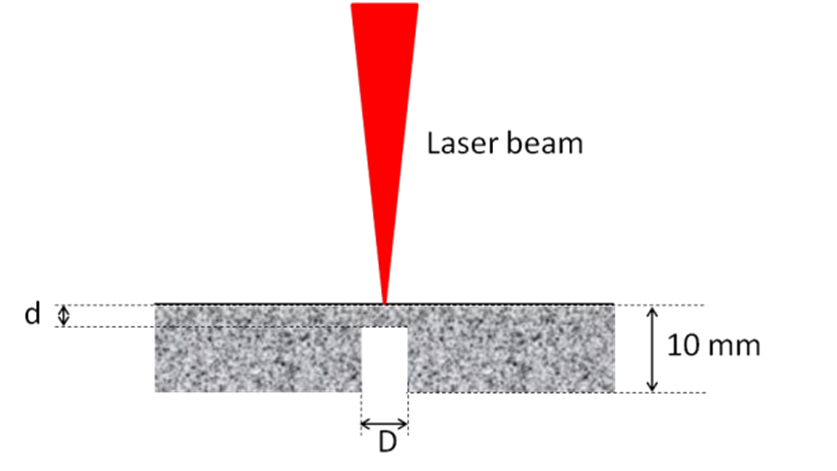
\includegraphics[width=0.3\linewidth]{./Figure/Figure2/a.png}}\hfill
	\subfigure[]{\label{subfig:2b}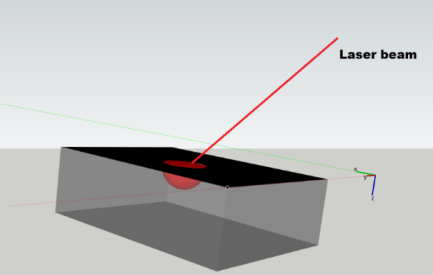
\includegraphics[width=0.3\linewidth]{./Figure/Figure2/b.png}} 
	\hspace*{\fill} \\ \hspace*{\fill}
	\subfigure[]{\label{subfig:2c}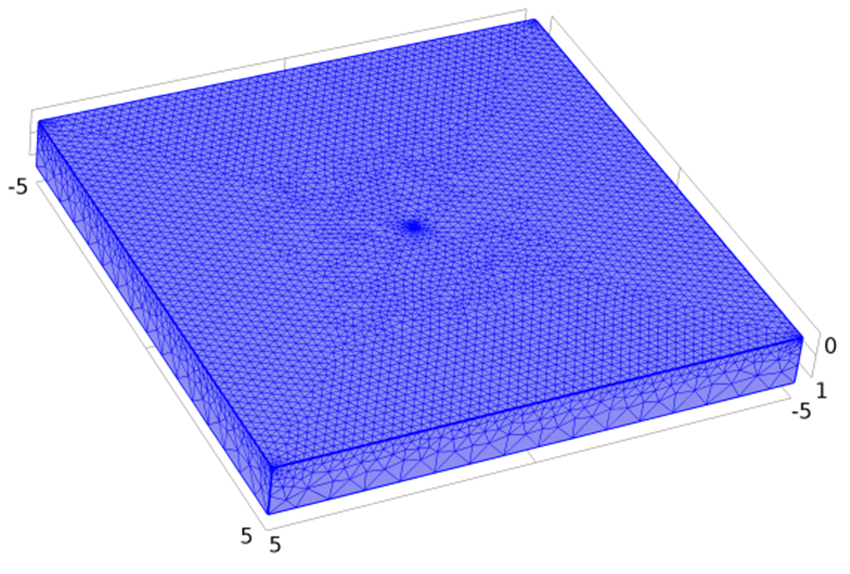
\includegraphics[width=0.3\linewidth]{./Figure/Figure2/c.png}}\hfill
	\subfigure[]{\label{subfig:2d}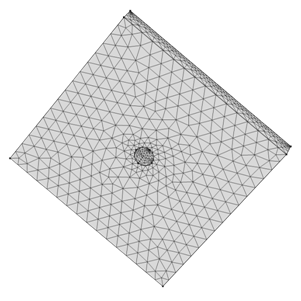
\includegraphics[width=0.3\linewidth]{./Figure/Figure2/d.png}}
	\hspace*{\fill}
    
	
		\caption{(a) Cross-sectional view of the geometry - (b) 3D Thermal response to a laser 
	excitation - (c) Geometry and meshing (front side), dimensions appears in cm  - (d) 
	Geometry and meshing (back side).}
  \label{fig:2}
\end{figure}


Furthermore, the black paint layer is considered as a dielectric material so that the energy provided by the interaction between the laser beam and material involves an absorption coefficient $\alpha$, near 1.
Transient conduction analysis of $heat$ $transfer$ $module$ has been selected to solve heat equation. The 2D geometry of the problem is represented in Fig.\,\ref{subfig:2a} where $d$ is the defect depth, $D$ is the defect diameter. Boundary condition imposed to all surfaces is in form of the following equation:

\begin{equation}
  \label{eq:33}
  n(k \nabla T) = \alpha q_0 + h(T_{ext} - T) \ ,
\end{equation}

\noindent where $n$ is the normal vector, $\alpha$ the absorption coefficient, $q_0$ is the inward heat flux on top surface and is equal to 0 on other surfaces, $h$ is a coefficient representing heat transfer losses due to convective heat flux with surrounding atmosphere. $h$ is equal to \SI{5}{\watt \per \square \metre \per \kelvin} on all surfaces, except on the surfaces of the defect where it is equal to 0 to simulate thermal insulation. $T_{ext}$ is the surrounding atmosphere temperature and it is assumed that the radiation heat transfer losses are neglected. 

For meshing, free tetrahedral meshes are selected with choice of a custom element size. The maximum element size is equal to \SI{0.032}{\milli \metre} with a maximum element growth rate equal to 1.35. The smallest element size is obtained near to the origin (0, 0, 0) centrally located on top of the surface (see Fig.\,\ref{subfig:2c}). A fine meshing is constructed with a number of elements ranging from $75,000$ to $225,000$ due to the presence of a \SI{0.1}{\milli \metre} layer on top of the simulated object surface. Furthermore, the system to solve consists of a number of degrees of freedom ranging from $111,000$ to $324,000$ and depends of the chosen geometry. Record time stepping is selected to \SI{0.1}{\second} in a range from \SI{0}{\second} to \SI{2}{\second}. Geometric Multigrid GMRES iterative linear solver is used. Backward Differentiation Formula (BDF) implicit method is used to help solver to converge.

	%

  \begin{figure}
  \centering
	

  \hspace*{\fill}
  \subfigure[]{\label{subfig:3a}\includegraphics[width=0.3\linewidth]{./Figure/Figure3/fig2d.png}} \hfill
  \subfigure[]{\label{subfig:3b}\includegraphics[width=0.3\linewidth]{./Figure/Figure3/fig2e.png}} 
  \subfigure[]{\label{subfig:3c}\includegraphics[width=0.3\linewidth]{./Figure/Figure3/fig2f.png}} 
	\hspace*{\fill} \\ \hspace*{\fill}
  \subfigure[]{\label{subfig:3d}\includegraphics[width=0.3\linewidth]{./Figure/Figure3/1.png}} \hfill
  \subfigure[]{\label{subfig:3e}\includegraphics[width=0.3\linewidth]{./Figure/Figure3/2.png}} 
  \subfigure[]{\label{subfig:3f}\includegraphics[width=0.3\linewidth]{./Figure/Figure3/3.png}} 
  \hspace*{\fill}
	
	  \caption{(a) and (d) Thermal response, observed on a non-defective area - (b) and (e) 
	Thermal response, observed on an area with defect of 1 mm below surface - (c) and (f) 
	Thermal response, 
	observed on an area with defect of 0.5 mm below surface.}
	
  \label{fig:3}
\end{figure}


  
  %\begin{figure}
  %\centering
  %\hspace*{\fill}
  %\subfigure[]{\label{subfig:3a}\includegraphics[width=0.3\linewidth]{fig2d.png}} \hfill
  %\subfigure[]{\label{subfig:3b}\includegraphics[width=0.3\linewidth]{fig2e.png}} 
  %\subfigure[]{\label{subfig:3c}\includegraphics[width=0.3\linewidth]{fig2f.png}} 
	%\hspace*{\fill} \\ \hspace*{\fill}
  %\subfigure[]{\label{subfig:3d}\includegraphics[width=0.3\linewidth]{1.png}} \hfill
  %\subfigure[]{\label{subfig:3e}\includegraphics[width=0.3\linewidth]{2.png}} 
  %\subfigure[]{\label{subfig:3f}\includegraphics[width=0.3\linewidth]{3.png}} 
  %\hspace*{\fill}
  %\caption{(a) and (d) Thermal response, observed on a non-defective area - (b) and (e) 
	%Thermal response, observed on an area with defect of 1 mm below surface - (c) and (f) 
	%Thermal response, 
	%observed on an area with defect of 0.5 mm below surface.}
  %\label{fig:3}
%\end{figure}


The interaction of the laser beam with the solid surface produces a thermal wave propagating through the solid media. In the case of a media without any defects and assuming a semi-infinite and isotropic solid, the thermal response is defined by the shape of a symmetric hemisphere\cite{Li2011} as shown in Fig.\,\ref{subfig:2b}. This response is modified due to the presence of a defect close to the excited area.

The simulation results are depicted in Fig.\,\ref{subfig:3a}-\ref{subfig:3b}-\ref{subfig:3c} by representing the temperature distribution in kelvin. It can be noted that the temperature intensity increases when the laser heats the defective area. Subsequently, the maximum temperature is reached for defects nearer to the surface. Fig.\,\ref{subfig:3d}-\ref{subfig:3e}-\ref{subfig:3f} represent the thermal response using another color-map. It can be observed that the amount of the thermal response increases due to the presence of inhomogeneities in the solid media.
	
\subsubsection{Defect detection algorithm}\label{subsec:312}
\graphicspath{{./Figure/Figure4/}}

%
\begin{figure}
  \centering



  % Define the properties of the different blocks
  \tikzstyle{module}=[draw, draw=blue!80, text width=10em, 
  text centered, minimum height=5em, minimum width = 15em, drop shadow, rounded corners,
  fill=blue!30]

  \tikzstyle{vecArrow} = [thick, decoration={markings,mark=at position
    1 with {\arrow[semithick]{open triangle 60}}},
  double distance=1.4pt, shorten >= 5.5pt,
  preaction = {decorate},
  postaction = {draw,line width=1.4pt, white,shorten >= 4.5pt}]

  % Define distances for bordering
  \def\blockdist{1.5}
  \def\edgedist{2.5}

  \begin{tikzpicture}[node distance=3cm,thick,scale=0.4, every node/.style={scale=0.4},path image/.style={
      path picture={
        \node at (path picture bounding box.center) {
          \includegraphics[width=1cm]{#1}
        };}}]
    \tikzstyle{conefill} = [path image=,fill opacity=0.8]

    % First block with the pre-processing
    \node[module=above:pre] (pre) at (4.5,-2.6) {\Large Background\\ Subtraction};
    \node[module,below of=pre] (seg) {\Large Noise\\ Reduction};
    \node[module,below of=seg] (reg) {\Large Contrast\\ Enhancement};
    \draw[->] (pre)--(seg);
    \draw[->] (seg)--(reg);
    \begin{pgfonlayer}{background}
      \path (pre.west |- pre.north)+(-0.9,1.0+\blockdist) node (a) {};
      \path (reg.east |- reg.south)+(+0.9,-0.5) node (b) {};
      
      \path[fill=blue!10,rounded corners, draw=blue!20, dashed] (a) rectangle (b);
    \end{pgfonlayer}
    \path (pre.north) +(0,+\blockdist) node (bgreg) {\Large Pre-processing};

    % Second block with the segmentation
    \begin{scope}[node distance=3cm]
      \node[module] (det) [right=0cm and 2cm of seg] {\Large Region\\Growing};
    \end{scope}
    \begin{pgfonlayer}{background}
      \path (det.west |- det.north)+(-0.9,1.0+\blockdist) node (c) {};
      \path (det.east |- det.south)+(+0.9,-0.5) node (d) {};
      \path[fill=blue!10,rounded corners, draw=blue!20, dashed] (c) rectangle (d);
    \end{pgfonlayer}

    \path (det.north) +(0,+\blockdist) node (bgreg) {\Large Segmentation};

    % % Define the place where the arrow should start anf finish
    % \path (seg.east |- seg.north)+(+0.9,0) node (e) {};
    % \path (det.west |- seg.north)+(-0.8,0) node (f) {};

    % \draw[double distance =3pt,preaction={-triangle 90,thin,draw,shorten >=-1mm}] (e) -- (f) node[midway,above] {\Large Regularized data};

    % Third block with the merging
    \begin{scope}[node distance=3cm]
      \node[module] (mer) [right=0cm and 2cm of det] {\Large Merging};
    \end{scope}
    \node[module,below of=mer] (bin) {\Large Binarization};
    \begin{pgfonlayer}{background}
      \path (mer.west |- mer.north)+(-0.9,1.0+\blockdist) node (c) {};
      \path (bin.east |- bin.south)+(+0.9,-0.5) node (d) {};
      \path[fill=blue!10,rounded corners, draw=blue!20, dashed] (c) rectangle (d);
    \end{pgfonlayer}

    \path (mer.north) +(0,+\blockdist) node (bgreg) {\Large Detection};

    \draw[->] (mer)--(bin);

    \begin{scope}[yshift=-170,xshift=950]
      \transparent{1.0}\draw[path image=defect.png] (0,0) rectangle (1.0,1.0);
      \path (0,0)+(0.5,1.6) node {\Large Det. Img.};
    \end{scope}

    \begin{scope}[yshift=-132,xshift=594]
      \transparent{0.6}\draw[path image=rg.png] (0,0) rectangle (1.0,1.0);
    \end{scope}

    \begin{scope}[yshift=-136,xshift=600]
      \transparent{0.6}\draw[path image=rg.png] (0,0) rectangle (1.0,1.0);
    \end{scope}

    \begin{scope}[yshift=-140,xshift=606]
      \transparent{0.8}\draw[path image=rg.png] (0,0) rectangle (1.0,1.0);
      \path (0,0)+(0.0,1.8) node {\Large Seg. Img.};
    \end{scope}

    \begin{scope}[yshift=-132,xshift=270]
      \transparent{0.6}\draw[path image=th_im.png] (0,0) rectangle (1.0,1.0);
    \end{scope}

    \begin{scope}[yshift=-136,xshift=276]
      \transparent{0.6}\draw[path image=th_im.png] (0,0) rectangle (1.0,1.0);
    \end{scope}

    \begin{scope}[yshift=-140,xshift=282]
      \transparent{0.8}\draw[path image=th_im.png] (0,0) rectangle (1.0,1.0);
      \path (0,0)+(0.0,1.8) node {\Large Enh. Img.};
    \end{scope}

    \begin{scope}[yshift=-166,xshift=-82]
      \transparent{0.6}\draw[path image=th_im_2.png] (0,0) rectangle (1.0,1.0);
    \end{scope}

    \begin{scope}[yshift=-172,xshift=-76]
      \transparent{0.6}\draw[path image=th_im_2.png] (0,0) rectangle (1.0,1.0);
    \end{scope}

    \begin{scope}[yshift=-176,xshift=-70]
      \transparent{0.8}\draw[path image=th_im_2.png] (0,0) rectangle (1.0,1.0);
      \path (0,0)+(0.0,1.8) node {\Large Thermal Image};
    \end{scope}

    \path (seg.west |- seg.north)+(-2.5,-1) node (i) {};
    \path (seg.west |- seg.north)+(-0.9,-1) node (j) {};
    \draw[double distance =3pt,preaction={-triangle 90,thin,draw,shorten >=-1mm}] (i) -- (j);
    
    \path (seg.east |- seg.north)+(0.9,-1) node (ii) {};
    \path (det.west |- det.north)+(-0.9,-1) node (jj) {};
    \draw[double distance =3pt,preaction={-triangle 90,thin,draw,shorten >=-1mm}] (ii) -- (jj);

    \path (det.east |- det.north)+(0.9,-1) node (ii) {};
    \path (mer.west |- mer.north)+(-0.9,-1) node (jj) {};
    \draw[double distance =3pt,preaction={-triangle 90,thin,draw,shorten >=-1mm}] (ii) -- (jj);

    \path (mer.east |- mer.north)+(0.9,-1) node (ii) {};
    \path (mer.east |- mer.north)+(2.5,-1) node (jj) {};
    \draw[double distance =3pt,preaction={-triangle 90,thin,draw,shorten >=-1mm}] (ii) -- (jj);   
    
  \end{tikzpicture}



  \caption{Image processing work-flow to detect non-through defects.}
  \label{fig:wkdetection}
\end{figure}


The object surface is punctually scanned using a laser beam and at each of these scans, a thermal image is acquired (see Fig.\,\ref{subfig:44c}).
Defect localization is characterized by a change of the heat distribution and therefore can be detected with an appropriate image processing algorithm in the thermal images.
Our developed framework is depicted in Fig.\,\ref{fig:wkdetection} and can be subdivided into three stages: (i) pre-processing, (ii) segmentation, and (iii) detection.

\paragraph{Pre-processing} Each acquired thermal image is enhanced by successively subtracting the background, reducing the noise, and stretching the contrast. The background to be subtracted consists in the acquisition of a thermal image before laser stimulation. Additionally, a median filtering is applied to the image to reduce the noise and the denoised image is enhanced through contrast stretching.
\paragraph{Segmentation} Then, the enhanced image is segmented using the region growing segmentation algorithm~\cite{Adams1994}. 
The initial seed point is automatically placed on the center of the thermal response corresponding to the maximum temperature in the image.
Then, the region grows if the difference of temperature values of the neighboring pixels and the region's mean is less than a given region membership criterion.
The pixel with the smallest difference is assigned to the segmented region.
\paragraph{Detection} The detection is subdivided into two stages: (i) merging and (ii) binarization.
All segmented images are combined together by creating a matrix $s$ such that the number of white pixels of a given segmented image is assigned to the location $(i,j)$, which corresponds to the location of the laser stimulation.
Subsequently, to limit the influence of the emissivity change and detect robustly the defective area, the median $\tilde{s}$ is computed for each \ac{roi} with a size $(40\times40)$ and compared to each value $s(i,j)$ inside this \ac{roi} in order to binarize $s$:

\begin{equation}
  \label{eq:3}
s_m(i,j) = \begin{cases}
1 & \quad \text{if } s(i,j) \geq K \times \tilde{s}\\
0 & \quad \text{if } s(i,j) < K \times \tilde{s}
\end{cases}
\end{equation}

\noindent where $K > 1$ and $s_m(i,j)$ is the resulting binary mask of the defects detection.
If $K \gg 1$, the defect detection is more robust to noise. However, only shallowest defect are detected; if $K \to 1$, the defect detection is subject to noise. However, deeper defect are detected.

\subsection{Fiber orientation assessment}\label{subsec:32}

	%
\graphicspath{{./Figure/Figure5/}}
\begin{figure}
  \centering
	
  % Define the properties of the different blocks
  \tikzstyle{module}=[draw, draw=blue!80, text width=10em, 
  text centered, minimum height=5em, minimum width = 15em, drop shadow, rounded corners,
  fill=blue!30]

  \tikzstyle{vecArrow} = [thick, decoration={markings,mark=at position
    1 with {\arrow[semithick]{open triangle 60}}},
  double distance=1.4pt, shorten >= 5.5pt,
  preaction = {decorate},
  postaction = {draw,line width=1.4pt, white,shorten >= 4.5pt}]

  % Define distances for bordering
  \def\blockdist{1.5}
  \def\edgedist{2.5}

  \begin{tikzpicture}[node distance=3cm,thick,scale=0.4, every node/.style={scale=0.4},path image/.style={
      path picture={
        \node at (path picture bounding box.center) {
          \includegraphics[width=1cm]{#1}
        };}}]
    \tikzstyle{conefill} = [path image=,fill opacity=0.8]

    % First block with the pre-processing
    %\node[module=above:pre] (pre) at (4.5,-2.6) {\Large Background\\ Subtraction};
    \node[module=above:seg] (seg) at (4.5,-2.6) {\Large Background\\ Subtraction};
    %\node[module,below of=seg] (reg) {\Large Contrast\\ Enhancement};
    %\draw[->] (pre)--(seg);
    %\draw[->] (seg)--(reg);
    \begin{pgfonlayer}{background}
      \path (seg.west |- seg.north)+(-0.9,1.0+\blockdist) node (a) {};
      \path (seg.east |- seg.south)+(+0.9,-0.5) node (b) {};
      
      \path[fill=blue!10,rounded corners, draw=blue!20, dashed] (a) rectangle (b);
    \end{pgfonlayer}
    \path (pre.north) +(0,+\blockdist) node (bgreg) {\Large Pre-processing};

    % Second block with the segmentation
    \begin{scope}[node distance=3cm]
      \node[module] (det) [right=0cm and 2cm of seg] {\Large Region\\Growing};
    \end{scope}
    \node[module,below of=det] (can) {\Large Canny\\ Edge Detector};
    \begin{pgfonlayer}{background}
      \path (det.west |- det.north)+(-0.9,1.0+\blockdist) node (c) {};
      \path (can.east |- can.south)+(+0.9,-0.5) node (d) {};
      \path[fill=blue!10,rounded corners, draw=blue!20, dashed] (c) rectangle (d);
    \end{pgfonlayer}

    
    \draw[->] (det)--(can);

    \path (det.north) +(0,+\blockdist) node (bgreg) {\Large Segmentation};

    % % Define the place where the arrow should start anf finish
    % \path (seg.east |- seg.north)+(+0.9,0) node (e) {};
    % \path (det.west |- seg.north)+(-0.8,0) node (f) {};

    % \draw[double distance =3pt,preaction={-triangle 90,thin,draw,shorten >=-1mm}] (e) -- (f) node[midway,above] {\Large Regularized data};

    % Third block with the merging
    \begin{scope}[node distance=3cm]
      \node[module] (mer) [right=0cm and 2cm of det] {\Large Algebraic\\ Fitting};
    \end{scope}
    \begin{pgfonlayer}{background}
      \path (mer.west |- mer.north)+(-0.9,1.0+\blockdist) node (c) {};
      \path (mer.east |- mer.south)+(+0.9,-0.5) node (d) {};
      \path[fill=blue!10,rounded corners, draw=blue!20, dashed] (c) rectangle (d);
    \end{pgfonlayer}

    \path (mer.north) +(0,+\blockdist) node (bgreg) {\Large Fitting};

    \begin{scope}[yshift=-85,xshift=950]
      \transparent{1.0}\draw[path image=fig9d.png] (0,0) rectangle (1.0,1.0);
      \path (0,0)+(0.5,1.6) node {\Large Det. Img.};
    \end{scope}

    \begin{scope}[yshift=-60,xshift=606]
      \transparent{1.0}\draw[path image=fig9c.png] (0,0) rectangle (1.0,1.0);
      \path (0,0)+(0.0,1.8) node {\Large Seg. Img.};
    \end{scope}

    \begin{scope}[yshift=-60,xshift=282]
      \transparent{1.0}\draw[path image=th_im.png] (0,0) rectangle (1.0,1.0);
      \path (0,0)+(0.0,1.8) node {\Large Enh. Img.};
    \end{scope}

    \begin{scope}[yshift=-85),xshift=-70]
      \transparent{1.0}\draw[path image=th_im_2.png] (0,0) rectangle (1.0,1.0);
      \path (0,0)+(0.0,1.8) node {\Large Thermal Image};
    \end{scope}

    \path (seg.west |- seg.north)+(-2.5,-1) node (i) {};
    \path (seg.west |- seg.north)+(-0.9,-1) node (j) {};
    \draw[double distance =3pt,preaction={-triangle 90,thin,draw,shorten >=-1mm}] (i) -- (j);
    
    \path (seg.east |- seg.north)+(0.9,-1) node (ii) {};
    \path (det.west |- det.north)+(-0.9,-1) node (jj) {};
    \draw[double distance =3pt,preaction={-triangle 90,thin,draw,shorten >=-1mm}] (ii) -- (jj);

    \path (det.east |- det.north)+(0.9,-1) node (ii) {};
    \path (mer.west |- mer.north)+(-0.9,-1) node (jj) {};
    \draw[double distance =3pt,preaction={-triangle 90,thin,draw,shorten >=-1mm}] (ii) -- (jj);

    \path (mer.east |- mer.north)+(0.9,-1) node (ii) {};
    \path (mer.east |- mer.north)+(2.5,-1) node (jj) {};
    \draw[double distance =3pt,preaction={-triangle 90,thin,draw,shorten >=-1mm}] (ii) -- (jj);   
    
  \end{tikzpicture}

  
	\caption{Image processing work-flow to infer the fiber orientation.}
  \label{fig:wkfiber}
\end{figure}

%%% Local Variables:
%%% mode: latex
%%% TeX-master: "../../../master"
%%% End:


The fiber orientation is estimated based on the pulsed thermal ellipsometry approach~\cite{Cielo1987}.
Indeed, the thermal response of a polymer matrix composite material stimulated by a laser beam is elliptic due to the propagation of the heat through the fiber.
The framework developed to infer the fiber orientation is depicted in Fig.\,\ref{fig:wkfiber}.
Thermal images are acquired with an IR camera and are pre-processed with the following steps: (i) background subtraction, (ii) a segmentation using region growing, and (iii) an edge detection using Canny edge detector~\cite{Canny1986}. 
Three methods are commonly used to fit an ellipse: (i) algebraic fitting~\cite{Fitzgibbon1999}, (ii) orthogonal least squares fitting~\cite{Ahn2001}, and (iii) Maximum Likelihood algorithms~\cite{Chojnacki2000}. 
The two latter methods are suitable for 3D data, whereas the first method can only be applied to 2D problems.
Algebraic fitting, however, offers a low computational complexity and is suitable in our case.
In this method, the ellipse is formulated by the general conic polynomial:

\begin{equation}
  \label{eq:4}
  F(a, X) = aX = 0 \,
\end{equation}

\noindent with 

\begin{eqnarray}
  a & = & \begin{bmatrix} A & B & C & D & E & F \\ \end{bmatrix}^\intercal \nonumber\\
  X & = & \begin{bmatrix} x^2 & xy & y^2 & x & y & 1 \\ \end{bmatrix}^\intercal \nonumber
\end{eqnarray}

The fitting is performed by a least square minimization of the Euclidean distances such that:

\begin{equation}
  \argmin{a} \sum_{i=1}^{n} \left( A x_i^2 + B x_i y_i + C y_i^2 + D x_i + E Y_i + F \right)^2 \ .
\end{equation}

The following constraint yields to one solution which corresponds to an ellipse:

\begin{equation}
  4AC - B^2 = 1 \ .
\end{equation}
